\newpage

\section{Architettura}

\subsubsection{Informazioni generali}
\label{Architettura}
\begin{figure}[ht]
	\centering
	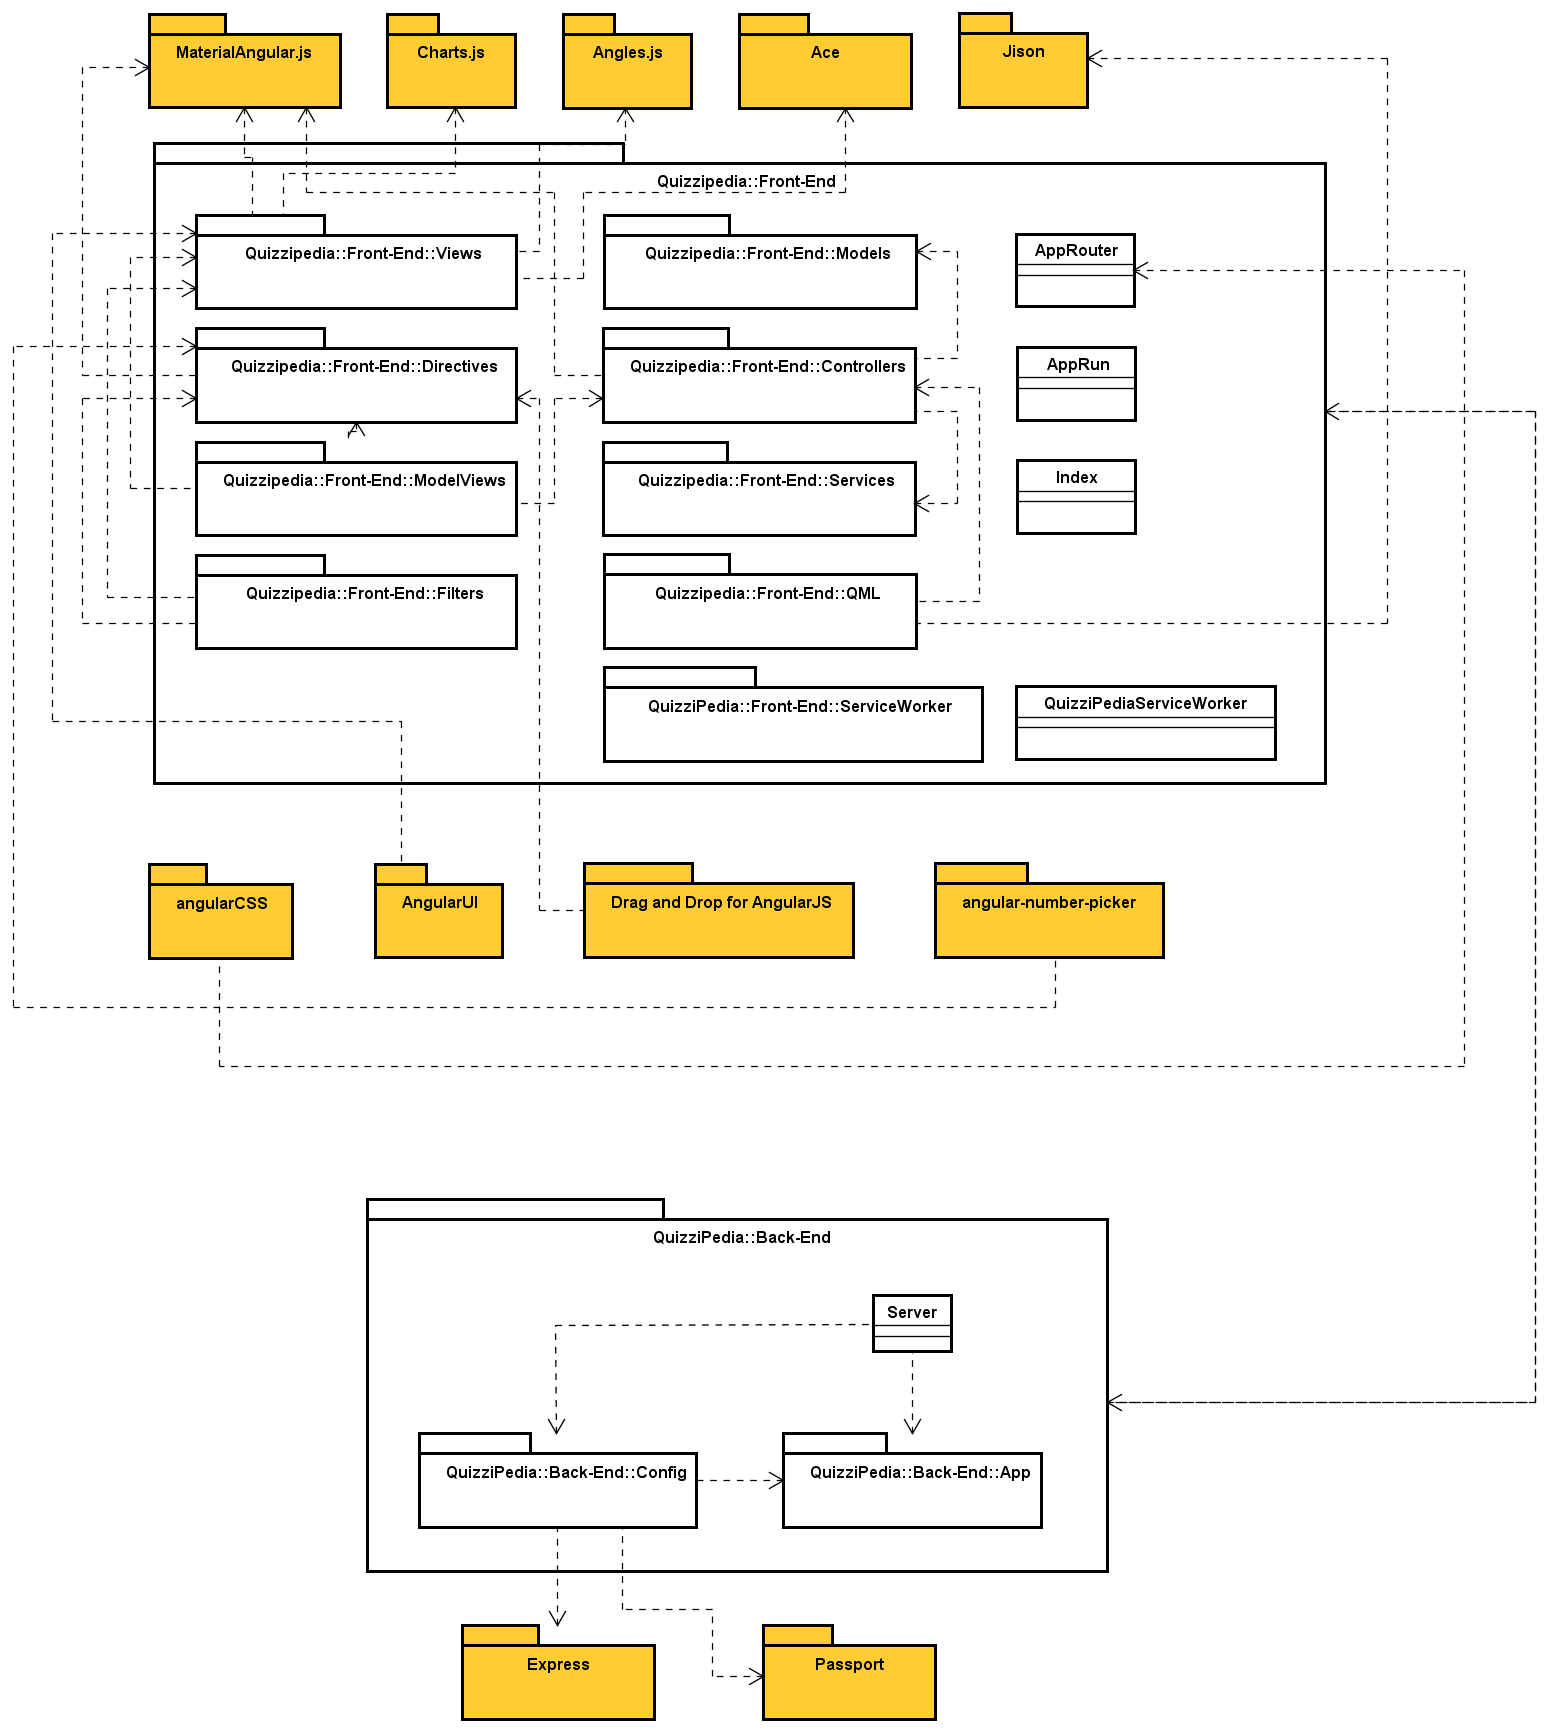
\includegraphics[scale=0.35]{UML/Package/QuizziPedia.png}
	\caption{Architettura}
\end{figure}
\FloatBarrier
\begin{itemize}
	\item \textbf{Descrizione}: architettura ad alto livello dell'applicazione \progetto;
	\item \textbf{Packages contenuti}:
	\begin{itemize}
		\item \texttt{QuizziPedia::Front-End}: \textit{package\ped{G}} contenente i \textit{packages\ped{G}} che compongono il Front-End;
		\item \texttt{QuizziPedia::Back-End}: \textit{package\ped{G}} contenente i \textit{packages\ped{G}} che compongono il Back-End;
	\end{itemize}
	\item \textbf{Librerie e framework}:
	\begin{itemize}
		\item \texttt{MaterialAngular.js}
		\item \texttt{Charts.js}
		\item \texttt{Angles.js}
		\item \texttt{Ace}
		\item \texttt{Jison}
		\item \texttt{AngularCSS}
		\item \texttt{AngularUI}
		\item \texttt{Drag and Drop for AngularJS}
		\item \texttt{angular-number-picker}
		\item \texttt{Express}
		\item \texttt{Passport}
	\end{itemize}
\end{itemize}
